% Compile with pdflatex: pdflatex hand_gesture_presentation.tex
\documentclass{beamer}
\usetheme{Madrid}
\usepackage[utf8]{inputenc}
\usepackage[french]{babel}
\usepackage{graphicx}

% Increase title font size
\setbeamerfont{title}{size=\LARGE, series=\bfseries}

\title[Contrôle Gestuel]{Système de Contrôle Gestuel par Reconnaissance de Main}
\author{Réalisé par : My Name}
\date{}

\begin{document}



% Detailed Plan Slide with all slide titles and image placeholders
\begin{frame}{Plan détaillé}
\begin{itemize}
  \item \textbf{Couverture}\hfill

  \item \textbf{Intégration de MediaPipe Hands}\hfill
  \item \textbf{Capture vidéo avec OpenCV}\hfill
  \item \textbf{Collecte des données avec \texttt{data.py}}\hfill
  \item \textbf{Ajout de gestes aléatoires ("OTHER")}\hfill
  \item \textbf{Extraction des vecteurs de landmarks}\hfill
  \item \textbf{Normalisation des vecteurs}\hfill
  \item \textbf{Entraînement du classifieur}\hfill
  \item \textbf{Mapping vers des actions système}\hfill
\end{itemize}
\end{frame}

\section{Étapes Principales}

% Slide 1: Intégration MediaPipe
\begin{frame}{Intégration de MediaPipe Hands}
    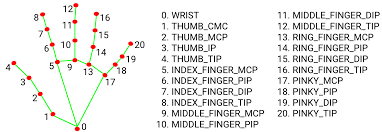
\includegraphics[height=3cm]{hand.png}

Configuration et installation du module "Hands" de MediaPipe pour détecter en temps réel 21 repères 3D de la main.
\end{frame}

% Slide 2: Capture OpenCV
\begin{frame}{Capture vidéo avec OpenCV}
Ouverture de la webcam, boucle de récupération d'images et gestion de l'arrêt par la touche Esc.
\end{frame}

% Slide 3: Collecte des données
\begin{frame}{Collecte des données avec \texttt{data.py}}
Enregistrement jusqu'à 1000 échantillons par geste et export des vecteurs de landmarks dans un fichier CSV.
\end{frame}

% Slide 4: Gestes aléatoires
\begin{frame}{Ajout de gestes aléatoires ("OTHER")} 
Capture de positions de main sans geste défini pour aider le modèle à différencier les commandes.
\end{frame}

% Slide 5: Extraction landmarks
\begin{frame}{Extraction des vecteurs de landmarks}
    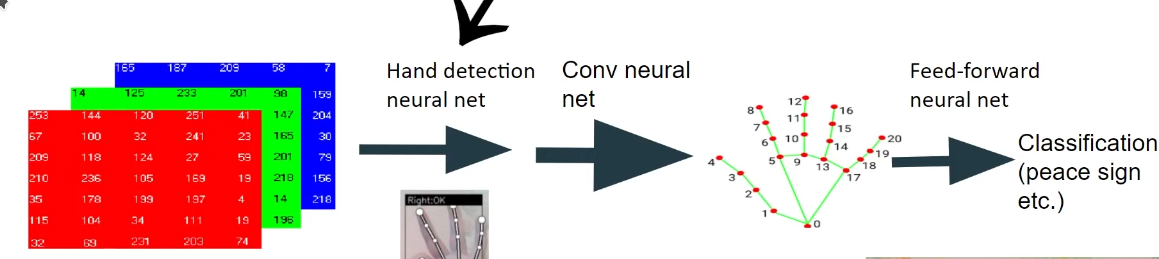
\includegraphics[height=2.5cm]{classification.png}
Aplatissement des 21 points (x, y, z) en un vecteur unidimensionnel.
\end{frame}

% Slide 6: Normalisation
\begin{frame}{Normalisation des vecteurs}

Ajustement des coordonnées par rapport au poignet pour une invariance à la position, à la taille et à la distance, améliorant robustesse et généralisation.
\end{frame}

% Slide 7: Entraînement du classifieur
\begin{frame}{Entraînement du classifieur}
Utilisation des vecteurs normalisés pour apprendre à reconnaître chaque geste.
\end{frame}

% Slide 8: Mapping actions
\begin{frame}{Mapping vers des actions système}

Chaque prédiction ("UP"/"DOWN"/"PINCH") déclenche respectivement l'augmentation, la diminution du volume ou la mise en sourdine de l'ordinateur.
\end{frame}

\end{document}
